\chapter{Resultados y discusión}

La esencia de esta tesis era la creación de un conjunto de programas de cómputo científico que calculan entalpías de formación de compuestos orgánicos a $T$ = 298 K partiendo de archivos de salida de \textbf{Gaussian09}. En consecuencia, es necesaria una explicación detallada de todo esto. Por lo que he dividido esta descripción en dos secciones; el algoritmo y su uso para la obtención de resultados. 

Es importante mencionar que los programas creados fueron inspirados por un programa de cómputo científico que también calcula entalpías de formación de compuestos orgánicos, dicho programa fue escrito en el lenguaje de \textbf{FORTRAN} en su versión 90, el autor fue el coasesor de esta tesis, \textbf{Dr. Julio Manuel Pérez Hernández}. La principal razón para crear nuevos programas en un lenguaje diferente es porque en un futuro se pretende extender el cálculo hacia otras propiedades termodinámicas haciendo uso de la programación orientada a objetos de \textbf{C++}. 

\section{Algoritmo (diseño del programa)}
La entalpía de formación fue calculada a partir del método de atomización \cite{Lewars2016} y varias correcciones térmicas de la energía interna \cite{Nicolaides1996}. La Termodinámica Estadística nos permitió separar la función de partición en un producto de los componentes traslacionales, rotacionales, vibracionales, electrónicas y nucleares, con la finalidad de obtener la función de estado de nuestro interés \cite{McQuarrie1976}. Todo ello culminó en la creación de varios programas de cómputo que automatizan el cálculo de entalpías de formación. Además, se produjeron versiones cuya arquitectura de \textit{software} permitirá en un futuro, añadir diferentes métodos de una manera rápida \cite{Curtiss2007, Simmie2015}. El procedimiento general se observa en el siguiente diagrama de flujo (véase la figura \ref{diagrama-flujo}). A continuación, se explica a detalle cada uno de los pasos del diagrama de flujo general junto con un ejemplo. Para esto, se eligió al metanol (figura \ref{metanol}), a la que nos referiremos desde ahora como \textbf{molécula X} ( Mol.X ).


\begin{figure}[hbtp]
\begin{center}
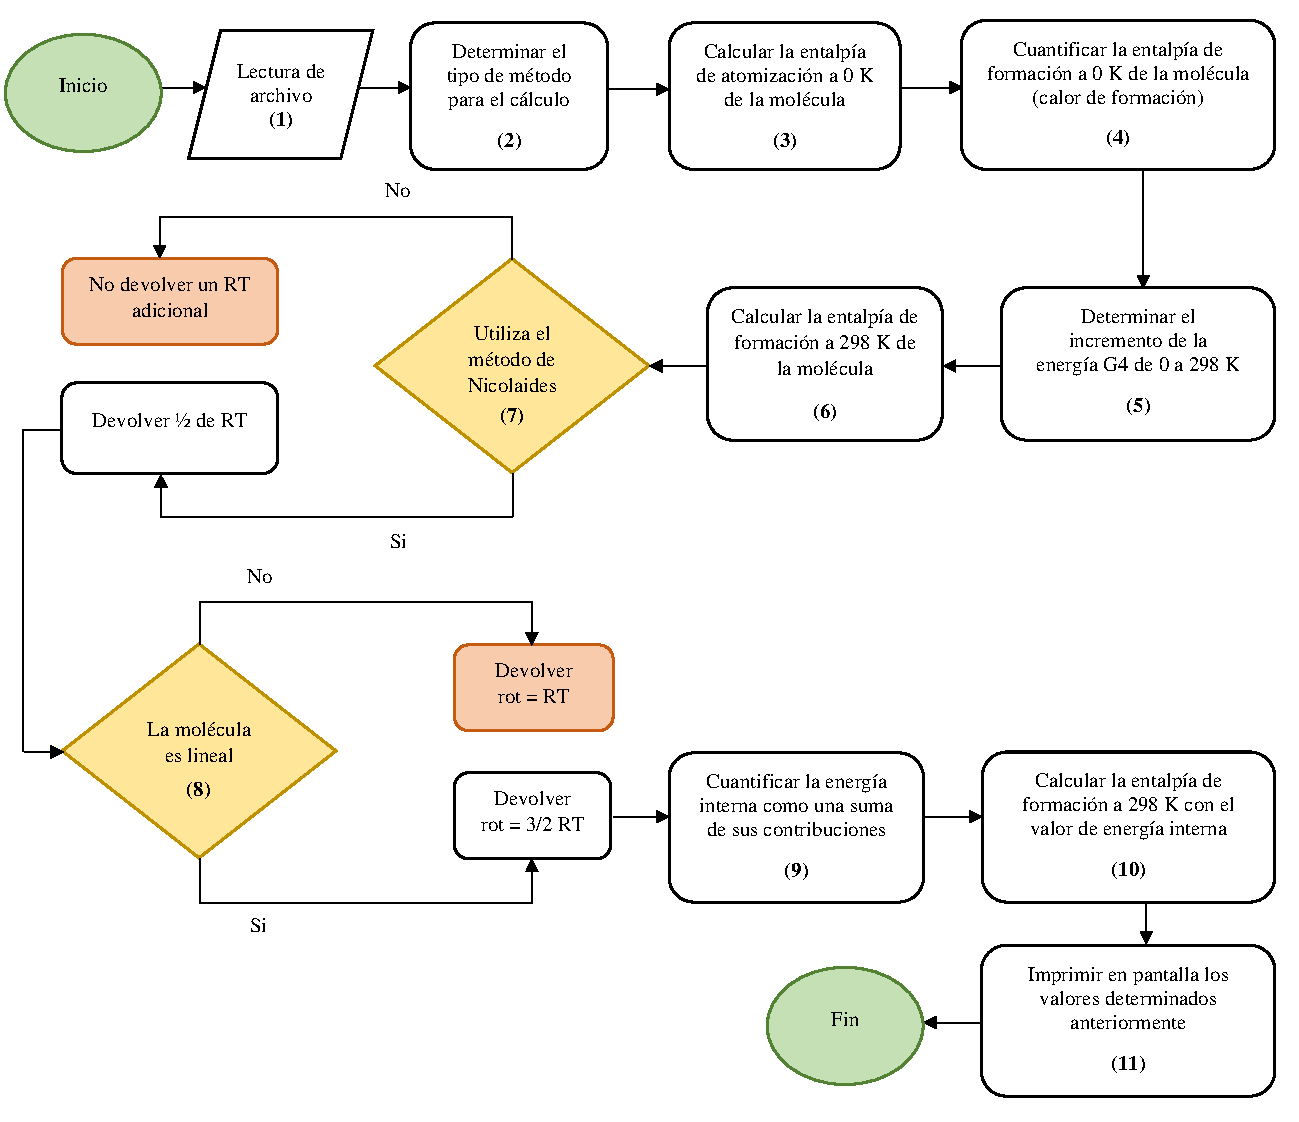
\includegraphics[width=\textwidth]{graphs/diagrama-flujo}
\caption{Diagrama de flujo general}
\label{diagrama-flujo}
\end{center}
\end{figure}


\begin{figure}[hbtp]
\begin{center}
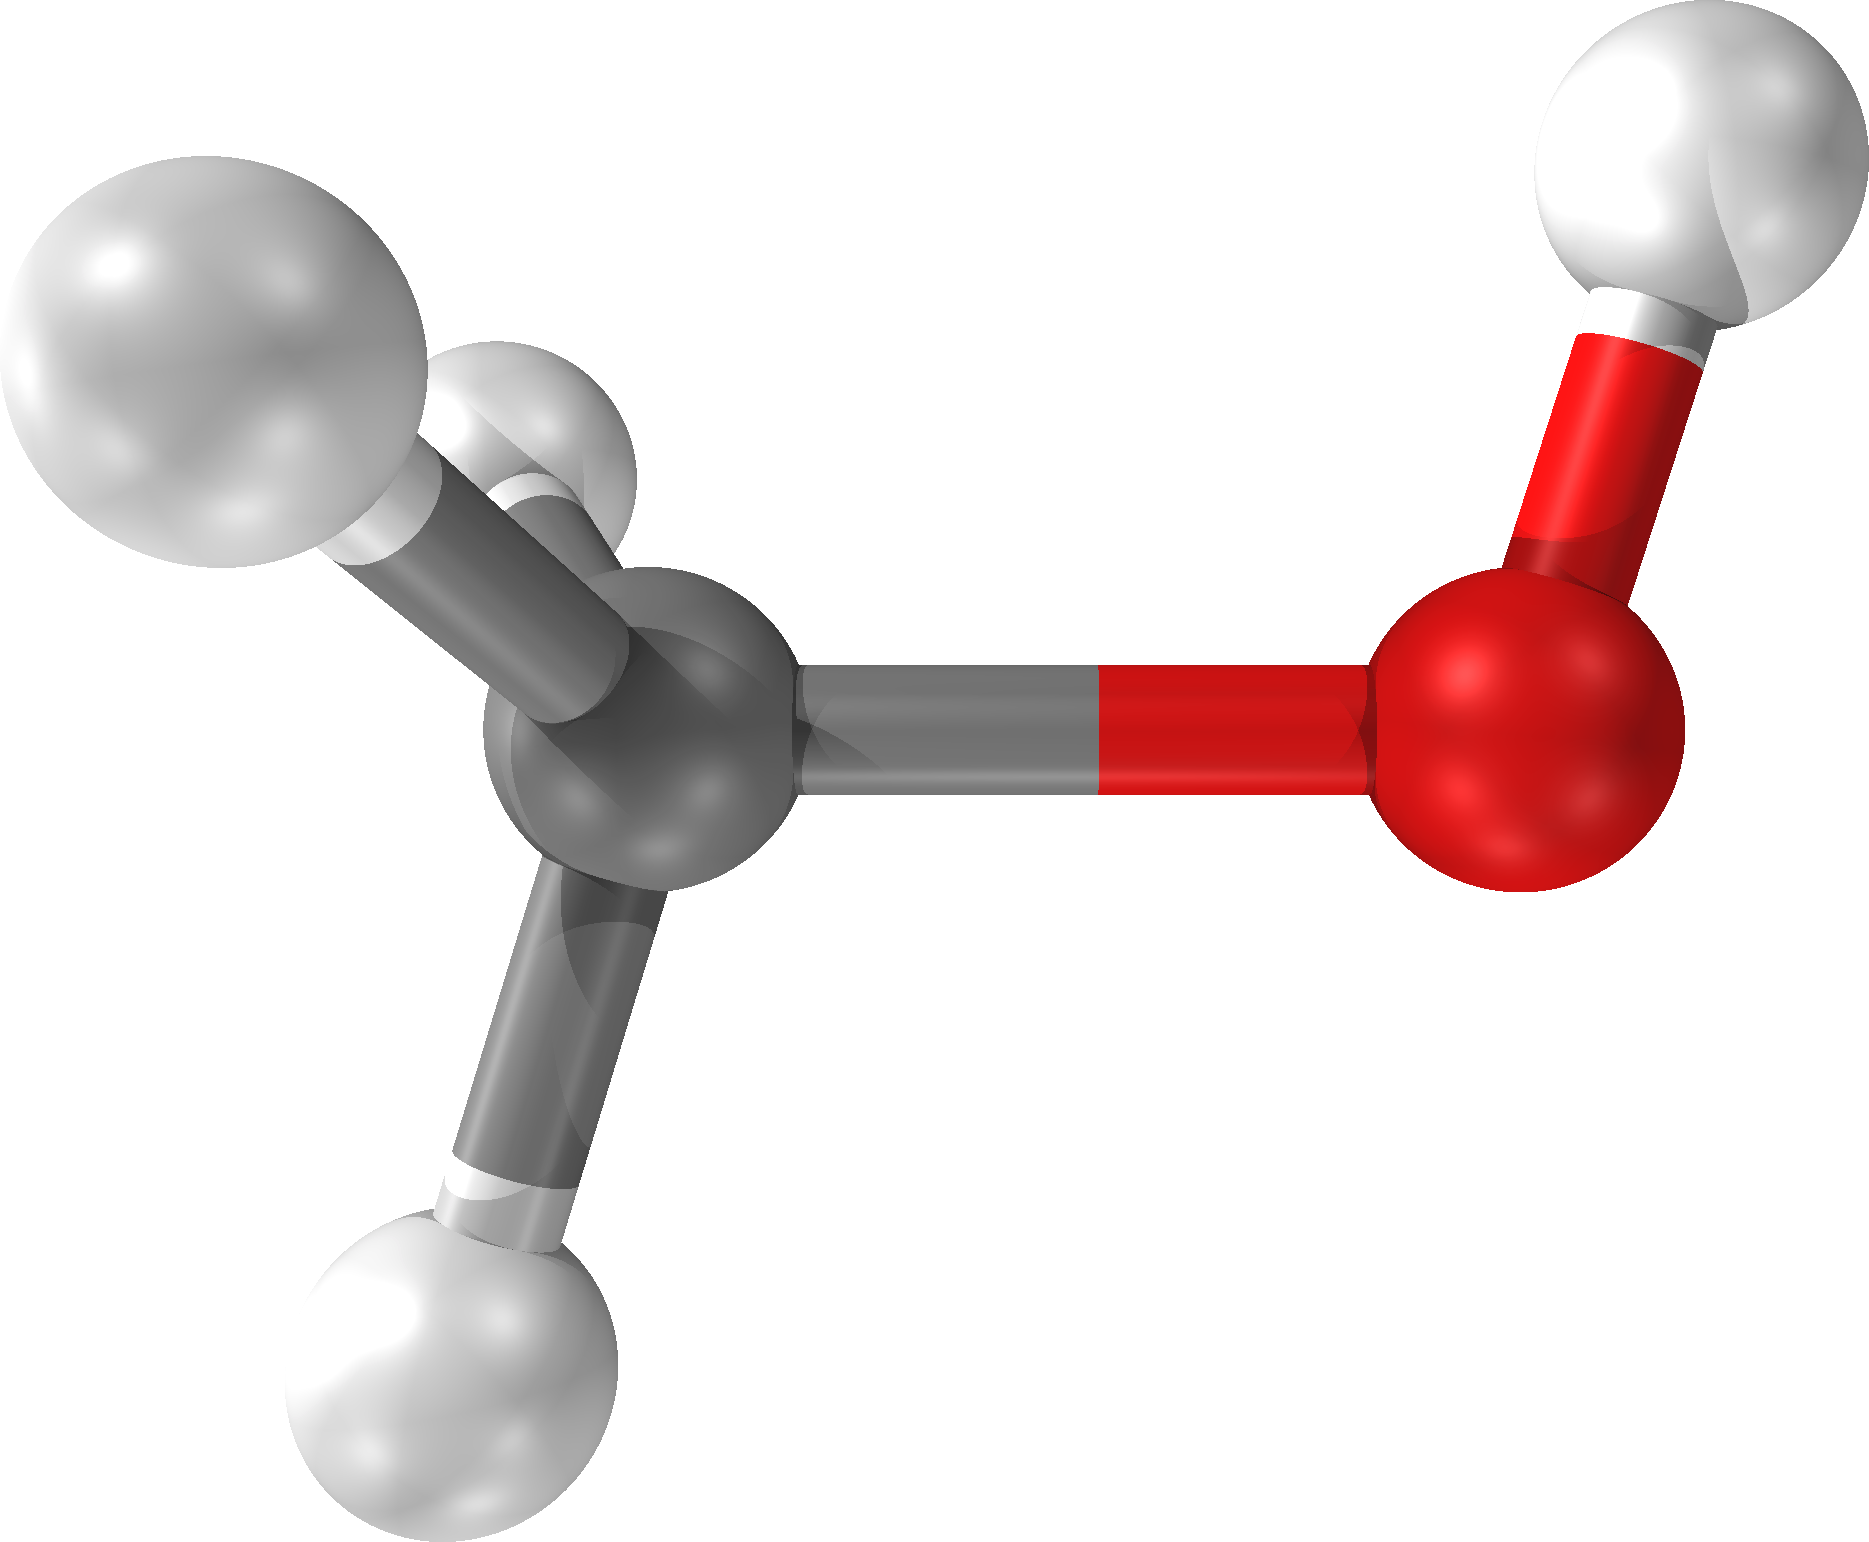
\includegraphics[scale=0.1]{graphs/metanol.png}
\caption{Molécula de metanol, utilizada para explicar el diagrama de flujo general.}
\label{metanol}
\end{center}
\end{figure}

\subsection {Inicio}

El programa comienza con la lectura de un archivo de entrada que contiene la información necesaria de la molécula. Para la \textbf{molécula X}, el archivo de entrada tendrá la siguiente forma:

\begin{lstlisting}[caption = Output de CH3OH-G4.txt]
G4
3
-115.651767
-115.647489
1 4
6 1
8 1
0
0
12
322.7598
1058.0227
1094.4693
1175.9092
1389.4710
1487.0775
1495.0437
1513.5228
2980.0300
3023.9572
3106.3296
3831.1143
\end{lstlisting}



\subsection{Paso 1 del diagrama de flujo general}

Ahora, se leerá el archivo de entrada de la siguiente forma:
\begin{multicols}{2}
\begin{enumerate}		
	\item Categoría de método. 
	\item Número de especies atómicas.
	\item Energía G4 a 0 K.
	\item Entalpía G4 a 0 K.
	\item Número atómico y número de átomos.
	\item Tipo de molécula (lineal o no lineal).
	\item Modelo de aproximación usada (Nicolaides o Rotor Rígido/Oscilador Armónico).
	\item Número de modos de vibración.
	\item Frecuencias vibracionales de la molécula.
\end{enumerate}
\end{multicols}

Las líneas 1, 2, 3, 4 y 5 siempre se encargarán de leer la categoría del método, el número de especies atómicas, la energía G4 a $T$ = 0, la entalpía G4 a $T$ = 0, el número atómico y el número de átomos, respectivamente. Mientras que las líneas 6, 7, 8 y 9 no siempre ocuparán el mismo lugar, porque éstas dependen de líneas anteriores.\\

\newpage

Por ejemplo, para la \textbf{molécula X}, el número de especies atómicas serán tres: Hidrógeno, Carbono y Oxígeno. En consecuencia, la línea 5 se repetirá tres veces para las especies mencionadas. Después, se leerá el tipo de molécula (lineal o no lineal), posteriormente, el modelo de aproximación usada (Nicolaides o Rotor Rígido/Oscilador Armónico). Por último, el número de modos de vibración que influirá en las frecuencias vibracionales de la molécula. Al terminar el proceso de lectura, toda esta información es almacenada en variables específicas del programa. 

 
\subsection{Paso 2 del diagrama de flujo general}

Como tercer paso en el diagrama general, se encuentra la determinación del método utilizado, que es indispensable para comenzar con los cálculos. \textbf{EnthalpyNIST} (uno de los 3 programas creados) cuenta con varios métodos de Gaussian, pero en nuestra explicación utilizaremos sólo el método \textbf{G4 de Gaussian09} (véase el apéndice B para obtener información sobre otros métodos de Gaussian). Hecho esto, el programa tiene la certeza de qué datos ocupar para las especies atómicas antes leídas.



\subsection{Paso 3 del diagrama de flujo general}

En este paso se realiza el cálculo de la entalpía de atomización a $T$ = 0 de la molécula. Aquí se utilizan los valores del método G4 para cada uno de los átomos presentes en la \textbf{molécula X}, la cantidad estequiométrica de estos y la entalpía G4 de la molécula a $T$ = 0 (véase las ecuaciones \ref{eq:4.1} y \ref{eq:4.2}). Para concluir, se realiza una conversión de unidades de energía (hartree a kJ). Obsérvese las ecuaciones \ref{eq:4.4} y \ref{eq:4.5}.

\begin{equation}
	\Delta_\mathrm{{a}} H^{\circleddash}_{\mathrm{0}}\mathrm{(CH_3OH) = \Delta E^\mathrm{{total}}_{0K} (C(^{3}P) + 4H(^{2}S) + O(^{3}S))- \Delta E^\mathrm{{total}}_{0K} (CH_{3}OH)}
\label{eq:4.1}
\end{equation}

\begin{equation}
	\Delta_\mathrm{{a}} H^{\circleddash}_{0}\mathrm{(CH_3OH) = -37.834170\;\mathrm{h} + 4(-0.501420)\;\mathrm{h} - 75.045500\;\mathrm{h} -(-115.651767)\;\mathrm{h}}
\label{eq:4.2}
\end{equation}

\begin{equation}
	\Delta_\mathrm{{a}} H^{\circleddash}_{0}\mathrm{(CH_3OH) = -114.88535\;\mathrm{h} + 115.651767\;\mathrm{h}}
\end{equation}

\begin{equation}
	\Delta_\mathrm{{a}} H^{\circleddash}_{0}\mathrm{(CH_3OH) = (\;0.766417\;\mathrm{h})(2625.4997480\;\mathrm{kJ\;mol^{-1})}}
\label{eq:4.4}
\end{equation}

\begin{equation}
	\Delta_\mathrm{{a}} H^{\circleddash}_{0}\mathrm{(CH_3OH) = 2012.22764\; \mathrm{kJ\;mol^{-1}}}
\label{eq:4.5}
\end{equation}
 
\subsection{Paso 4 del diagrama de flujo general}

En este paso se realiza el cálculo de la entalpía de formación a $T$ = 0 de la molécula. Nuevamente, se utilizan valores experimentales para cada uno de los átomos presentes en la molécula junto con su cantidad específica y el valor de la entalpía de atomización a $T$ = 0 obtenido anteriormente (ecuaciones \ref{eq:4.6} y \ref{eq:4.7}). Al valor obtenido en este paso se le conoce como \textbf{calor de formación} (ecuación \ref{eq:4.9}). Por último, se realiza una conversión de unidades de energía (kJ a kcal), ver las ecuaciones \ref{eq:4.10} y \ref{eq:4.11}. 

\begin{equation}
	\Delta_\mathrm{{f}} H^{\circleddash}_{0}\mathrm{(CH_3OH) = \Delta_{f} H^{\circleddash}_{0}(C(^{3}P) + 4H(^{2}S) + O(^{3}S))- \Delta_{f} H^{\circleddash}_{0} (CH_{3}OH)}
\label{eq:4.6}
\end{equation}

\begin{multline}
	\Delta_\mathrm{{f}} H^{\circleddash}_{0}\mathrm{(CH_3OH)} = 711.185\;\mathrm{kJ\;mol^{-1}} + 4(216.03500)\mathrm{kJ\;mol^{-1}} +...\\
	...\; 246.7900\;\mathrm{kJ\;mol^{-1}} - 2012.22764\; \mathrm{kJ\;mol^{-1}}
\label{eq:4.7}
\end{multline}

\begin{equation}
	\Delta_\mathrm{{f}} H^{\circleddash}_{0}\mathrm{(CH_3OH) = 1822.115 - 2012.22764\; kJ\;mol^{-1}}
\end{equation}

\begin{equation}
	\Delta_\mathrm{{f}} H^{\circleddash}_{0}\mathrm{(CH_3OH) = -190.11264\; kJ\;mol^{-1}}
\label{eq:4.9}
\end{equation}

\begin{equation}
	\Delta_\mathrm{{f}} H^{\circleddash}_{0}\mathrm{(CH_3OH) = (-190.11264\; kJ\;mol^{-1})(0.23888\; kcal)}
\label{eq:4.10}
\end{equation}

\begin{equation}
	\Delta_\mathrm{{f}} H^{\circleddash}_{0}\mathrm{(CH_3OH) = -\;45.41\;kcal}
\label{eq:4.11}
\end{equation}


\subsection{Paso 5 del diagrama de flujo general}

El paso 5 se encarga de cuantificar la diferencia entre las  dos cantidades G4 ($T$ = 0 y $T$ = 298 K) leídas en el paso 1 (ecuación \ref{eq:4.13}). Además, se realiza una conversión de unidades de energía (hartree a kJ), ecuaciones \ref{eq:4.14} y \ref{eq:4.15}.

\begin{equation}
	\Delta \Delta H^{\circleddash}\mathrm{(CH_3OH) = G4\;\textrm{Entalpía} - G4\;(0\;K)}
\label{eq:4.12}
\end{equation}

\begin{equation}
	\Delta \Delta H^{\circleddash}\mathrm{(CH_3OH) = -115.647489\;\mathrm{h} - (-115.651767)\;h}
\label{eq:4.13}
\end{equation}

\begin{equation}
	\Delta \Delta H^{\circleddash}\mathrm{(CH_3OH) = (0.004278\;\mathrm{h})(2625.4997480\; kJ\;mol^{-1})}
\label{eq:4.14}
\end{equation}

\begin{equation}
	\Delta \Delta H^{\circleddash}\mathrm{(CH_3OH) = 11.23188\;kJ\;mol^{-1}}
\label{eq:4.15}
\end{equation}


\subsection{Paso 6 del diagrama de flujo general}

En el paso 6 se obtiene el valor de la entalpía de formación a $T$ = 298 K (sumando el calor de formación, la diferencia de las dos cantidades G4 y restando los incrementos correspondientes para los elementos de la molécula en sus estados estándar), en consecuencia, se usan los valores obtenidos en los pasos 4 y 5 (véase las ecuaciones \ref{eq:4.16}, \ref{eq:4.17}, \ref{eq:4.18} y \ref{eq:4.19}). Finalmente, se realiza una conversión de unidades de energía de kJ a kcal (ecuaciones \ref{eq:4.20} y \ref{eq:4.21}).

\begin{multline}
	\enthalpy*(f){}(CH_3OH) = \Delta_\mathrm{{f}} H^{\circleddash}_{0}\mathrm{(CH_{3}OH)} + \Delta \Delta H^{\circleddash} \mathrm{(CH_{3}OH)} \\ - (\Delta \Delta H^{\circleddash} \mathrm{(C)} + 2 \Delta \Delta H^{\circleddash}\mathrm{(H_{2})} + \frac{1}{2} \Delta \Delta H^{\circleddash}\mathrm{(O_{2}))}
\label{eq:4.16}
\end{multline}

\begin{multline}
	\enthalpy*(f){}\mathrm{(CH_3OH)} = -190.11264\;\mathrm{kJ\;mol^{-1}} + 11.23188\;\mathrm{kJ\;mol^{-1}}  \\ - (1.05100 + 2(8.46700) + \frac{1}{2} (8.67000))\mathrm{\; kJ\;mol^{-1}}
\label{eq:4.17}
\end{multline}

\begin{equation}
	\enthalpy*(f){}\mathrm{(CH_3OH) = -190.11264\;\mathrm{kJ\;mol^{-1}} + 11.23188\;\mathrm{kJ\;mol^{-1}} - 22.3265\;kJ\;mol^{-1}}
\label{eq:4.18}
\end{equation}

\begin{equation}
	\enthalpy*(f){}\mathrm{(CH_3OH) = -201.21\;kJ\;mol^{-1}}
\label{eq:4.19}
\end{equation}

\begin{equation}
	\enthalpy*(f){}\mathrm{(CH_3OH) = (-201.21 kJ\;mol^{-1})(0.23888 \:kcal)}
\label{eq:4.20}
\end{equation}

\begin{equation}
	\enthalpy*(f){}\mathrm{(CH_3OH) = -\;48.06 \:kcal}
\label{eq:4.21}
\end{equation}


\subsection{Paso 7, 8 y 9 del diagrama de flujo general}

Los pasos 7 y 8 son de los más importantes del programa, porque calculan la energía interna (paso 6) usando ecuaciones que provienen de la Termodinámica Estadística. Se inicia con dos sentencias de condición que evalúan parámetros de la molécula, como son:

\begin{multicols}{2}
\begin{enumerate}
	\item Aproximaciones a usar.
	\item El número de modos de vibración.
	\item Frecuencias vibracionales.
	\item Si es lineal o no.
\end{enumerate}
\end{multicols}

El tipo de aproximación usada solo puede tener dos valores, 0 y 1. Si el archivo de entrada de la molécula muestra un valor de 0 significa que se usará la aproximación de Nicolaides \textit{et al.} \cite{Nicolaides1996} (no toma en cuenta las frecuencias vibraciones de la molécula menores a 260 cm$^{-1}$ y devuelve $\frac{1}{2}$ de $RT$ para la contribución vibracional por cada frecuencia que sea menor a 260 cm$^{-1}$). Y si el valor es 1, la aproximación de rotor rígido y oscilador armónico \cite{McQuarrie1976} sera usada para los cálculos. 

También existen dos posibles valores en el archivo de entrada para el parámetro de la linealidad de la molécula. Un valor de 1 devolverá un $RT$ en la contribución rotacional, en cambio, si el valor es 0, el condicional retornará un $\frac{3}{2}$ de $RT$ en la contribución rotacional. Después, se inicia una estructura de control que se repetirá el mismo número de veces que el número de modos de vibración de la molécula (una molécula que tiene $N$ especies atómicas puede tener solamente $3N-6$ modos fundamentales de vibración para una molécula no lineal, o $3N-5$ si la molécula es lineal). \\

La iteración usa las ecuaciones \ref{eq:3.27}, \ref{eq:3.28}, \ref{eq:3.29}, \ref{eq:3.30} y \ref{eq:3.31} que provienen de la Termodinámica Estadística \cite{McQuarrie1976, Irikura1998} ,para determinar a la energía interna como una suma de las contribuciones vibracionales, rotacionales, traslacionales y electrónicas (ecuación \ref{eq:3.31}). La contribuci\'{o}n traslacional siempre tendr\'{a} el valor de $\frac{3}{2} RT$ para cualquier mol\'{e}cula (ecuación \ref{eq:3.27}). Adem\'{a}s, se agrega un $RT$ adicional a la energ\'{i}a interna para convertir la energía en entalpía (el llamado término $pV$, ecuación \ref{eq:3.29}). Cabe aclarar que el valor obtenido en la primera iteración es acumulativo para los subsecuentes. Concluida la determinación, se devuelve la suma total de la energía interna. Para la \textbf{molécula X} el número de modos de vibración será 12 (es una molécula no lineal), por lo consiguiente, la ecuación \ref{eq:3.30} se repetirá 12 veces con cada una de las frecuencias de la molécula. El resultado final es la suma de las contribuciones de la energía interna, véase la ecuación \ref{eq:3.31}.

\begin{multline}
	[H(298.15)-H(0)]= 1315.1747\;\mathrm{kJ\;mol^{-1}} + 3718.4568\;\mathrm{kJ\;mol^{-1}} +...\\...\; 3718.4568\;\mathrm{kJ\;mol^{-1}} + 2478.9712\;\mathrm{kJ\;mol^{-1}} = \mathrm{11.2310\;kJ\;mol^{-1}}
\label{eq:4.22}
\end{multline}

\newpage

\subsection{Paso 10 del diagrama de flujo general}

El paso 10 simplemente remplaza el valor obtenido anteriormente (energía interna), por el valor calculado en el paso 5 en la determinación de la entalpía de formación a $T$ = 298 K, es decir, en el paso 6. Para terminar, se hace una conversión de unidades de energía (kJ a kcal).


\begin{equation}
	\enthalpy*(f){}\mathrm{(CH_3OH) = -190.1126\;\mathrm{kJ\;mol^{-1}} + 11.2310\;\mathrm{kJ\;mol^{-1}} - 22.3265\;kJ\;mol^{-1}}
\label{eq:4.23}
\end{equation}

\begin{equation}
	\enthalpy*(f){}\mathrm{(CH_3OH) = -201.21\;kJ\;mol^{-1}}
\label{eq:4.24}
\end{equation}


\begin{equation}
	\enthalpy*(f){}\mathrm{(CH_3OH) = -\;48.06\;kcal}
\label{eq:4.25}
\end{equation}

\newpage

\subsection{Paso 11 del diagrama de flujo general}
El último paso del diagrama de flujo, se encarga de devolver los valores calculados anteriormente, imprimiéndolos en la pantalla a través de la línea de comandos de la siguiente forma:

\begin{lstlisting}[caption = Output de CH3OH-G4.txt en EnthalpyNIST]
$./computeEnthalpyNIST.x  CH3OH-G4.txt$
========================================================================
          New calculation of molecular enthalpies of formation

      Enthalpies of formation of gaseous atoms at 0 and thermal 
   corrections for elements in their standard state at 298 K from:

            NIST-JANAF Thermochemical Tables J. Physics Chem. 
                    Data Monograph 9, 1998, 1-1951.
========================================================================
Heats of formation:
0K          -190.11 kJ mol-1
0K          -45.41 kcal mol-1

Using Nicolaides method:
298K        -201.21 kJ mol-1
298K        -48.06 kcal mol-1

Using G4: 
298K        -201.21 kJ mol-1
298K        -48.06 kcal mol-1
========================================================================
\end{lstlisting}

\section{Código}
El lenguaje de programación elegido para crear de estos programas es C++. El motivo principal de su uso fue que facilita una programación orientada a objetos que fragmenta el código en partes independientes, permitiendo así, reciclar el código para futuros proyectos \cite{cplusplus2005, Deitel2014, Pitt2017}.

\subsection*{Clases}
Ahora, se enlistan los nombres de las clases utilizadas para estos programas:
\begin{multicols}{2}
\begin{itemize}
	\item Enthalpyinputdata.
	\item Method.
	\item EnthalpyG4.
	\item EnthalpyG3.
	\item EnthalpyG3MP2.
	\item EnthalpyCBS-APNO.
	\item EnthalpyCBS-QB3.
\end{itemize}
\end{multicols}

\subsection*{Clase Enthalpyinputdata}
Enthalpyinputdata se encarga de leer los datos (provenientes de Gaussian) del archivo de entrada. Los datos que lee esta clase son:
\begin{multicols}{2}
\begin{itemize}
	\item Tipo de método.
	\item Número de especies atómicas.
	\item Energía G4 a 0 K.
	\item Entalpía G4 a 0 K.
	\item Número atómico y número de átomos .
	\item Tipo de molécula (lineal o no lineal).
	\item Tipo de aproximación usada (Nicolaides o Rotor Rígido y Oscilador Armónico).
	\item Número de modos de vibración.
	\item Frecuencias vibracionales de la molécula.
\end{itemize}
\end{multicols}
La finalidad de esta clase es determinar y almacenar la información indispensable para comenzar con el cálculo de la entalpía de formación \cite{Pitt2017}. 

\subsection*{Clase Method}
La clase Method se utiliza para seleccionar el tipo de método que se realizó en Gaussian, y así, devolver valores específicos para los átomos de Hidrógeno, Carbono, Oxígeno, Nitrógeno, Flúor y Azufre.

\subsection*{Clases EnthalpyG4 y variantes}
El trabajo de esta clase y sus variantes (EnthalpyG3, EnthalpyG3MP2, EnthalpyCBS-APNO y EnthalpyCBS-QB3) es realizar las operaciones aritméticas para obtener el calor de formación de la molécula, la entalpía de formación a $T$ = 298 K mediante el método de atomización y la entalpía de formación a $T$ = 298 K con correcciones en la energía interna. Para concluir, imprime los resultados a través de la línea de comandos.

\newpage

\section{Conjunto de pruebas}

Como parte del proceso de diseño e implementación  de \textit{software} científico, es fundamental corroborar que los programas funcionan de forma correcta, por lo que se realizaron pruebas con moléculas que cuentan con entalpías de formación conocidas y que han sido reportadas en la literatura científica \cite{Ximello2020}. Las moléculas elegidas son isómeros del nitrobenzaladeído (figura \ref{n-NBA}) y son:

\begin{itemize}
\item 2-nitrobenzaldeh\'{i}do (2NBA).
\item 3-nitrobenzaldeh\'{i}do (3NBA).
\item 4-nitrobenzaldeh\'{i}do (4NBA).
\end{itemize}

Los derivados de nitrobenzaladeh\'{i}do son compuestos aromáticos que tienen un gran número de aplicaciones. Entre ellos se encuentran los intermediarios en la preparación de productos químicos de alto valor agregado, pesticidas, materiales ópticos no lineales, productos farmacéuticos, bases de Schiff, etcétera \cite{Ximello2020}.

\begin{figure}[hbtp]
\begin{center}
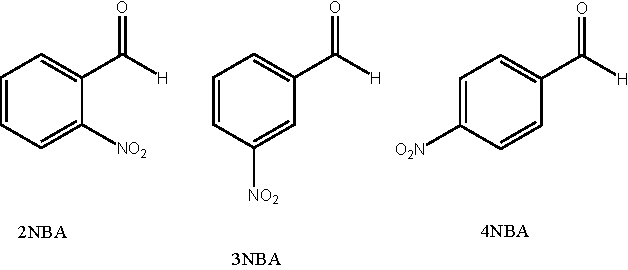
\includegraphics[width=\textwidth]{graphs/n-NBA.pdf}
\caption{Estructuras moleculares de 2-nitrobenzaldeh\'{i}do (2NBA), 3-nitrobenzaldeh\'{i}do (3NBA) y 4-nitrobenzaldeh\'{i}do (4NBA).}
\label{n-NBA}
\end{center}
\end{figure}

Las entalpías de formación de las moléculas fueron calculadas utilizando los métodos G4 y G3MP2, así mismo, se utilizaron las aproximaciones de oscilador armónico/rotor rígido \cite{McQuarrie1976} y Nicolaides \textit{et al.}\cite{Nicolaides1996} en todas las moléculas. Para ello, las frecuencias se calcularon a un nivel teórico B3LYP/6-31G(2df,p) escaladas a 0.9854 y 0.89290. Las entalpías atómicas de formación  fueron a $T$ = 0 y sus correcciones térmicas a $T$ = 298 K se tomaron de la referencia \cite{NIST1998} (excluyendo el valor del átomo de Carbono, cuyo dato coincide con Tajti \textit{et al.} \cite{Tajti2004} para el método G4). Los archivos de salida proceden del \textit{software} \textbf{Gaussian09}, mientras que el archivo que contiene la información necesaria para nuestro programa fue obtenida por el script \textbf{\textit{gendeltahfinputfile}} (proveniente del \textbf{Laboratorio de Fisicoquímica Orgánica Teórica de la BUAP}). Los valores de la entalpía de formación a $T$ = 298 K calculados por nuestro programa del 2-nitrobenzaldehído (2NBA), 3-nitrobenzaldehído (3NBA) y 4-nitrobenzaldehído (4NBA) se muestran a continuación.

\subsection{Conjunto de pruebas: 2NBA, 3NBA y 4NBA}

Es posible apreciar la entalpía de formación a $T$ = 298 K de las 15 simulaciones realizadas en las líneas 22, 20 y 21 de cada molécula, respectivamente. Todos los resultados coinciden con los valores de las moléculas de 2NBA, 3NBA y 4NBA reportados por Ximello \textit{et al.} \cite{Ximello2020}, véase las tablas \ref{Ximello-table-1}, \ref{Ximello-table-2} y \ref{Ximello-table-3}.  

\newpage

%2NBALa-2.txt
\begin{lstlisting}[caption = Output de 2NBALa-2.txt en EnthalpyTajti]
./computeEnthalpyTajti.x 2NBALa-2.txt
========================================================================
           New calculation of molecular enthalpies of formation                         
                                                                                                   
Enthalpies of formation of gaseous atoms at 0 (with the exception of 
carbon data 711.79 kJ/mol from A. Tajti et al. J. Chem. Phys. 121, 
2004, 11599) and thermal corrections for elements in their standard 
states at 298 K from:                   
                                                                                                   
NIST-JANAF Thermochemical Tables J. Physics Chem. Data Monograph 9, 1998,
 1-1951.
========================================================================
Heats of formation:
0K          -8.58 kJ mol-1
0K          -2.05 kcal mol-1

Using Nicolaides method:
298K        -30.82 kJ mol-1
298K        -7.36 kcal mol-1

Using G4 Enthalpy:
298K        -28.19 kJ mol-1
298K        -6.73 kcal mol-1
========================================================================
\end{lstlisting}

\newpage

%2NBALb-2.txt
\begin{lstlisting}[caption = Output de 2NBALb-2.txt en EnthalpyTajti]
./computeEnthalpyTajti.x 2NBALb-2.txt
========================================================================
           New calculation of molecular enthalpies of formation                         
                                                                                                   
Enthalpies of formation of gaseous atoms at 0 (with the exception of 
carbon data 711.79 kJ/mol from A. Tajti et al. J. Chem. Phys. 121, 
2004, 11599) and thermal corrections for elements in their standard 
states at 298 K from:                   
                                                                                                   
NIST-JANAF Thermochemical Tables J. Physics Chem. Data Monograph 9, 1998,
 1-1951.
========================================================================
Heats of formation:
0K          -16.26 kJ mol-1
0K          -3.88 kcal mol-1

Using Nicolaides method:
298K        -38.73 kJ mol-1
298K        -9.25 kcal mol-1

Using G4 Enthalpy:
298K        -36.25 kJ mol-1
298K        -8.66 kcal mol-1
========================================================================
\end{lstlisting}

\newpage

%3NBALa-2.txt
\begin{lstlisting}[caption = Output de 3NBALa-2.txt en EnthalpyTajti]
./computeEnthalpyTajti.x 3NBALa-2.txt
========================================================================
           New calculation of molecular enthalpies of formation                         
                                                                                                   
Enthalpies of formation of gaseous atoms at 0 (with the exception of 
carbon data 711.79 kJ/mol from A. Tajti et al. J. Chem. Phys. 121, 
2004, 11599) and thermal corrections for elements in their standard 
states at 298 K from:                   
                                                                                                   
NIST-JANAF Thermochemical Tables J. Physics Chem. Data Monograph 9, 1998,
 1-1951.
========================================================================
Heats of formation: 
0K          -35.36 kJ mol-1
0K          -8.45 kcal mol-1
                                                                                                   
Using Nicolaides method: 
298K        -57.82 kJ mol-1
298K        -13.81 kcal mol-1
                                                                                                   
Using G4 Enthalpy: 
298K        -55.46 kJ mol-1
298K        -13.25 kcal mol-1
========================================================================
\end{lstlisting}

\newpage

%3NBALb-2.txt
\begin{lstlisting}[caption = Output de 3NBALb-2.txt en EnthalpyTajti]
./computeEnthalpyTajti.x 3NBALb-2.txt
========================================================================
           New calculation of molecular enthalpies of formation                         
                                                                                                   
Enthalpies of formation of gaseous atoms at 0 (with the exception of 
carbon data 711.79 kJ/mol from A. Tajti et al. J. Chem. Phys. 121, 
2004, 11599) and thermal corrections for elements in their standard 
states at 298 K from:                   
                                                                                                   
NIST-JANAF Thermochemical Tables J. Physics Chem. Data Monograph 9, 1998,
 1-1951.
========================================================================
Heats of formation: 
0K          -33.75 kJ mol-1
0K          -8.06 kcal mol-1
                                                                                                   
Using Nicolaides method: 
298K        -56.26 kJ mol-1
298K        -13.44 kcal mol-1
                                                                                                   
Using G4 Enthalpy: 
298K        -53.82 kJ mol-1
298K        -12.85 kcal mol-1
========================================================================
\end{lstlisting}

\newpage

%4NBALa-2.txt
\begin{lstlisting}[caption = Output de 4NBALa-2.txt en EnthalpyTajti]
./computeEnthalpyTajti.x 4NBALa-2.txt
========================================================================
           New calculation of molecular enthalpies of formation                         
                                                                                                   
Enthalpies of formation of gaseous atoms at 0 (with the exception of 
carbon data 711.79 kJ/mol from A. Tajti et al. J. Chem. Phys. 121, 
2004, 11599) and thermal corrections for elements in their standard 
states at 298 K from:                   
                                                                                                   
NIST-JANAF Thermochemical Tables J. Physics Chem. Data Monograph 9, 1998,
 1-1951.
========================================================================
Heats of formation: 
0K          -33.82 kJ mol-1
0K          -8.08 kcal mol-1
                                                                                                   
Using Nicolaides method: 
298K        -56.33 kJ mol-1
298K        -13.45 kcal mol-1
                                                                                                   
Using G4 Enthalpy: 
298K        -53.84 kJ mol-1
298K        -12.86 kcal mol-1
========================================================================
\end{lstlisting}

%%%%%%%%%%%%%%%%%%%%%%%%%%%%%%%%%%%%%%%%%%1%%%%%%%%%%%%%%%%%%%%%%%%%%%%%%%%%%%%%%%%%%%%%%%%%%%%%%%%%%

\newpage

%2NBALa-2.txt
\begin{lstlisting}[caption = Output de 2NBALa-2.txt en EnthalpyNIST]
./computeEnthalpyNIST.x 2NBALa-2.txt
========================================================================
          New calculation of molecular enthalpies of formation

      Enthalpies of formation of gaseous atoms at 0 and thermal 
   corrections for elements in their standard state at 298 K from:

            NIST-JANAF Thermochemical Tables J. Physics Chem. 
                    Data Monograph 9, 1998, 1-1951.
========================================================================
Heats of formation:
0K          -16.61 kJ mol-1
0K          -3.97 kcal mol-1

Using Nicolaides method:
298K        -38.91 kJ mol-1
298K        -9.29 kcal mol-1

Using G3MP2 Enthalpy:
298K        -36.42 kJ mol-1
298K        -8.70 kcal mol-1
========================================================================
\end{lstlisting}

\newpage

%2NBALb-2.txt
\begin{lstlisting}[caption = Output de 2NBALb-2.txt en EnthalpyNIST]
./computeEnthalpyNIST.x 2NBALb-2.txt
========================================================================
          New calculation of molecular enthalpies of formation

      Enthalpies of formation of gaseous atoms at 0 and thermal 
   corrections for elements in their standard state at 298 K from:

            NIST-JANAF Thermochemical Tables J. Physics Chem. 
                    Data Monograph 9, 1998, 1-1951.
========================================================================
Heats of formation:
0K          -7.11 kJ mol-1
0K          -1.70 kcal mol-1

Using Nicolaides method:
298K        -29.28 kJ mol-1
298K        -6.99 kcal mol-1

Using G3MP2 Enthalpy:
298K        -26.60 kJ mol-1
298K        -6.35 kcal mol-1
========================================================================
\end{lstlisting}

\newpage

%3NBALa-2.txt
\begin{lstlisting}[caption = Output de 3NBALa-2.txt en EnthalpyNIST]
./computeEnthalpyNIST.x 3NBALa-2.txt
========================================================================
          New calculation of molecular enthalpies of formation

      Enthalpies of formation of gaseous atoms at 0 and thermal 
   corrections for elements in their standard state at 298 K from:

            NIST-JANAF Thermochemical Tables J. Physics Chem. 
                    Data Monograph 9, 1998, 1-1951.
========================================================================
Heats of formation:
0K          -35.18 kJ mol-1
0K          -8.40 kcal mol-1

Using Nicolaides method:
298K        -57.44 kJ mol-1
298K        -13.72 kcal mol-1

Using G3MP2 Enthalpy:
298K        -54.94 kJ mol-1
298K        -13.12 kcal mol-1
========================================================================
\end{lstlisting}

\newpage

%3NBALb-2.txt
\begin{lstlisting}[caption = Output de 3NBALb-2.txt en EnthalpyNIST]
./computeEnthalpyNIST.x 3NBALb-2.txt
========================================================================
          New calculation of molecular enthalpies of formation

      Enthalpies of formation of gaseous atoms at 0 and thermal 
   corrections for elements in their standard state at 298 K from:

            NIST-JANAF Thermochemical Tables J. Physics Chem. 
                    Data Monograph 9, 1998, 1-1951.
========================================================================
Heats of formation:
0K          -33.44 kJ mol-1
0K          -7.99 kcal mol-1

Using Nicolaides method:
298K        -55.77 kJ mol-1
298K        -13.32 kcal mol-1

Using G3MP2 Enthalpy:
298K        -53.19 kJ mol-1
298K        -12.70 kcal mol-1
========================================================================
\end{lstlisting}

\newpage

%4NBALa-2.txt
\begin{lstlisting}[caption = Output de 4NBALa-2.txt en EnthalpyNIST]
./computeEnthalpyNIST.x 4NBALa-2.txt
========================================================================
          New calculation of molecular enthalpies of formation

      Enthalpies of formation of gaseous atoms at 0 and thermal 
   corrections for elements in their standard state at 298 K from:

            NIST-JANAF Thermochemical Tables J. Physics Chem. 
                    Data Monograph 9, 1998, 1-1951.
========================================================================
Heats of formation:
0K          -33.23 kJ mol-1
0K          -7.94 kcal mol-1

Using Nicolaides method:
298K        -55.54 kJ mol-1
298K        -13.27 kcal mol-1

Using G3MP2 Enthalpy:
298K        -52.91 kJ mol-1
298K        -12.64 kcal mol-1
========================================================================
\end{lstlisting}

%%%%%%%%%%%%%%%%%%%%%%%%%%%%%%%%%%%%%%%%%%%%%%%%%%%%%%%%2%%%%%%%%%%%%%%%%%%%%%%%%%%%%%%%%%%%%%%%%%%%%%%%%%%%%%%%%%%%%%%%%%

\newpage

%2NBALa-2.txt
\begin{lstlisting}[caption = Output de 2NBALa-2.txt en EnthalpyArgonne]
./computeEnthalpyArgonne.x 2NBALa-2.txt
========================================================================
           New calculation of molecular enthalpies of formation                               
                                                                                                   
Enthalpies of formation of gaseous atoms at 0 and thermal corrections 
        for elements in their standard states at 298 K from:
                                                                                                                  
          
                    ARGONNE Thermochemical Tables                                    
                  Warning: sulfur is taken from NIST                                                                                                       
========================================================================
Heats of formation:
0K          -15.20 kJ mol-1
0K          -3.63 kcal mol-1

Using Nicolaides method:
298K        -37.49 kJ mol-1
298K        -8.96 kcal mol-1

Using G3MP2 Enthalpy:
298K        -35.01 kJ mol-1
298K        -8.36 kcal mol-1
========================================================================
\end{lstlisting}

\newpage

%2NBALb-2.txt
\begin{lstlisting}[caption = Output de 2NBALb-2.txt en EnthalpyArgonne]
./computeEnthalpyArgonne.x 2NBALb-2.txt
========================================================================
           New calculation of molecular enthalpies of formation                               
                                                                                                   
Enthalpies of formation of gaseous atoms at 0 and thermal corrections 
        for elements in their standard states at 298 K from:
                                                                                                                  
          
                    ARGONNE Thermochemical Tables                                    
                  Warning: sulfur is taken from NIST                                                                                                       
========================================================================
Heats of formation:
0K          -5.69 kJ mol-1
0K          -1.36 kcal mol-1

Using Nicolaides method:
298K        -27.86 kJ mol-1
298K        -6.65 kcal mol-1

Using G3MP2 Enthalpy:
298K        -25.19 kJ mol-1
298K        -6.02 kcal mol-1
========================================================================
\end{lstlisting}

\newpage

%3NBALa-2.txt
\begin{lstlisting}[caption = Output de 3NBALa-2.txt en EnthalpyArgonne]
./computeEnthalpyArgonne.x 3NBALa-2.txt
========================================================================
           New calculation of molecular enthalpies of formation                               
                                                                                                   
Enthalpies of formation of gaseous atoms at 0 and thermal corrections 
        for elements in their standard states at 298 K from:
                                                                                                                  
          
                    ARGONNE Thermochemical Tables                                    
                  Warning: sulfur is taken from NIST                                                                                                       
========================================================================
Heats of formation:
0K          -33.76 kJ mol-1
0K          -8.06 kcal mol-1

Using Nicolaides method:
298K        -56.02 kJ mol-1
298K        -13.38 kcal mol-1

Using G3MP2 Enthalpy:
298K        -53.52 kJ mol-1
298K        -12.78 kcal mol-1
========================================================================
\end{lstlisting}

\newpage

%3NBALb-2.txt
\begin{lstlisting}[caption = Output de 3NBALb-2.txt en EnthalpyArgonne]
./computeEnthalpyArgonne.x 3NBALb-2.txt
========================================================================
           New calculation of molecular enthalpies of formation                               
                                                                                                   
Enthalpies of formation of gaseous atoms at 0 and thermal corrections 
        for elements in their standard states at 298 K from:
                                                                                                                  
          
                    ARGONNE Thermochemical Tables                                    
                  Warning: sulfur is taken from NIST                                                                                                       
========================================================================
Heats of formation:
0K          -32.03 kJ mol-1
0K          -7.65 kcal mol-1

Using Nicolaides method:
298K        -54.35 kJ mol-1
298K        -12.98 kcal mol-1

Using G3MP2 Enthalpy:
298K        -51.78 kJ mol-1
298K        -12.37 kcal mol-1
========================================================================
\end{lstlisting}

\newpage

%4NBALa-2.txt
\begin{lstlisting}[caption = Output de 4NBALa-2.txt en EnthalpyArgonne]
./computeEnthalpyArgonne.x 4NBALa-2.txt
========================================================================
           New calculation of molecular enthalpies of formation                               
                                                                                                   
Enthalpies of formation of gaseous atoms at 0 and thermal corrections 
        for elements in their standard states at 298 K from:
                                                                                                                  
          
                    ARGONNE Thermochemical Tables                                    
                  Warning: sulfur is taken from NIST                                                                                                       
========================================================================
Heats of formation:
0K          -31.82 kJ mol-1
0K          -7.60 kcal mol-1

Using Nicolaides method:
298K        -54.12 kJ mol-1
298K        -12.93 kcal mol-1

Using G3MP2 Enthalpy:
298K        -51.50 kJ mol-1
298K        -12.30 kcal mol-1
========================================================================
\end{lstlisting}

%%%%%%%%%%%%%%%%%%%%%%%%%%%%%%%%%%%%%%%%%%%%%%%%%%%%%%%%%%%%%%%%%3%%%%%%%%%%%%%%%%%%%%%%%%%%%%%%%%%%%%%

%%%%%%%%%%%%%%%%%%%%%%%%%%%%%%%%%%%%%%%%%%%%%%%%%%%%%%%%%%%3%%%%%%%%%%%%%%%%%%%%%%%%%%%%%%%%%%%%%%%%%%%

\begin{table}[H]
\centering
\begin{tabular}{|c|c|c|}
\hline
	\multicolumn{3}{||c||}{$\enthalpy*(f){}(298.15 \mathrm{K})\; \mathrm{kJ\;mol^{-1}}$}\\
\hline
\hline
	n-NBA & Ximello \textit{et al.} \cite{Ximello2020} & EnthalpyTajti\\ 
\hline 
2NBAa & -28.19 & -28.19\\
\hline
2NBAb & -36.25 & -36.25\\ 
\hline 
3NBAa & -53.82 & -53.82\\
\hline
3NBAb & -55.46 & -55.46\\ 
\hline 
4NBAa & -53.84 & -53.84\\ 
\hline  
\end{tabular} 
	\caption[Entalpías de formación en fase gaseosa obtenidas mediante el método G4 de Gaussian de 2NBA, 3NBA y 4NBA a $T$ = 298 K y $p^{\circ}$ = 0.1 MPa, reportadas por Ximello \textit{et al.} \cite{Ximello2020}.] {Entalpías de formación en fase gaseosa obtenidas mediante el método G4 de Gaussian de 2NBA, 3NBA y 4NBA a $T$ = 298 K y $p^{\circ}$ = 0.1 MPa, reportadas por Ximello \textit{et al.} \cite{Ximello2020}. Obsérvese la segunda columna. Entalpías de formación en fase gaseosa obtenida por nuestro programa EnthalpyTajti, véase la tercer columna.}
\label{Ximello-table-1}
\end{table}

\begin{table}[H]
\centering
\begin{tabular}{|c|c|c|}
\hline
	\multicolumn{3}{||c||}{$\enthalpy*(f){}(298.15 \mathrm{K})\; \mathrm{kJ\;mol^{-1}}$}\\
\hline
\hline
	n-NBA & Ximello \textit{et al.} \cite{Ximello2020} & EnthalpyNIST\\ 
\hline 
2NBAa & -36.42 & -36.42\\
\hline
2NBAb & -26.60 & -26.60\\ 
\hline 
3NBAa & -54.94 & -54.94\\
\hline
3NBAb & -53.19 & -53.19\\ 
\hline 
4NBAa & -52.91 & -52.91\\ 
\hline  
\end{tabular} 
	\caption[Entalpías de formación en fase gaseosa obtenidas mediante el método G3MP2 de Gaussian de 2NBA, 3NBA y 4NBA a $T$ = 298 K y $p^{\circ}$ = 0.1 MPa, reportadas por Ximello \textit{et al.} \cite{Ximello2020}.] {Entalpías de formación en fase gaseosa obtenidas mediante el método G3MP2 de Gaussian de 2NBA, 3NBA y 4NBA a $T$ = 298 K y $p^{\circ}$ = 0.1 MPa, reportadas por Ximello \textit{et al.} \cite{Ximello2020}. Obsérvese la segunda columna. Entalpías de formación en fase gaseosa obtenida por nuestro programa EnthalpyNIST, véase la tercer columna.}
\label{Ximello-table-2}
\end{table}

\begin{table}[H]
\centering
\begin{tabular}{|c|c|c|}
\hline
	\multicolumn{3}{||c||}{$\enthalpy*(f){}(298.15 \mathrm{K})\; \mathrm{kJ\;mol^{-1}}$}\\
\hline
\hline
	n-NBA & Ximello \textit{et al.} \cite{Ximello2020} & EnthalpyArgonne\\ 
\hline
2NBAa & -35.01 & -35.01\\
\hline
2NBAb & -25.19 & -25.19\\ 
\hline 
3NBAa & -53.52 & -53.52\\
\hline
3NBAb & -51.78 & -51.78\\ 
\hline
4NBAa & -51.50 & -51.50\\ 
\hline  
\end{tabular} 
	\caption[Entalpías de formación en fase gaseosa obtenidas mediante el método G3MP2 de Gaussian de 2NBA, 3NBA y 4NBA a $T$ = 298 K y $p^{\circ}$ = 0.1 MPa, reportadas por Ximello \textit{et al.} \cite{Ximello2020}.]{Entalpías de formación en fase gaseosa obtenidas mediante el método G3MP2 de Gaussian de 2NBA, 3NBA y 4NBA a $T$ = 298 K y $p^{\circ}$ = 0.1 MPa, reportadas por Ximello \textit{et al.} \cite{Ximello2020}. Obsérvese la segunda columna. Entalpías de formación en fase gaseosa obtenida por nuestro programa EnthalpyArgonne, véase la tercer columna.}
\label{Ximello-table-3}
\end{table}

\newpage

Una de las razones para utilizar los valores de Tajti \textit{et al.} \cite{Tajti2004} es porque se subraya una ventaja relativa respecto al uso de una reacción elemental, específicamente en compuestos de referencia cuya entalpía de formación es cero por definición porque en cálculos extremadamente precisos evita errores asociados con las entalpías atómicas de formación para especies como el carbono o el flúor. Sin embargo, dado que no es posible hacer un cálculo de calor en un trozo de grafito, se propone un enfoque alternativo. Una de las referencias usadas fue el monóxido de carbono, su elección se debe a su entalpía de formación determinada experimentalmente (-113.81 $\pm$ 0.17 $\;\mathrm{kJ\;mol^{-1}}$ proveniente de las tablas termoquímicas de Rusic \textit{et al.} \cite{Ruscic2005}), esto no esta ligado hacía el átomo de carbono, por lo tanto, debería ser una referencia relativamente estable. Dado que los valores de CO y O ($\enthalpy*(f){}= 246.86 \pm 0.002\;\mathrm{kJ\;mol^{-1}}$), las energías de reacción elementales, deben ajustarse en 360.65 kJ mol$^{-1}$ por cada átomo de carbono para obtener entalpías de formación. Además los resultados que obtuvieron son sorprendentes, para los compuestos que tienen entalpías de formación bien establecidas y consistentes, según lo determinado por el enfoque ATcT de Ruscic \textit{et al.}\cite{Ruscic2005} los valores de calor determinados por el segundo método están dentro de 1 kJ mol$^{-1}$ en todos los casos. La asombrosa precisión de las entalpías de formación de los compuestos bien caracterizados en \cite{Tajti2004} sugiere que son mejores estimaciones que las que se encuentran en la base de datos NIST-JANAF \cite{NIST1998} para todos los compuestos restantes, excepto quizás el amoníaco.\\

Las 15 pruebas preliminares también se realizaron con el fin de reconocer posibles errores en los resultados durante la ejecución de los programas \textbf{EnthalpyTajti}, \textbf{EnthalpyNIST} y \textbf{EnthalpyArgonne}. No obstante, lo anterior sirve para confirmar que las comparación con Ximello \textit{et al.} \cite{Ximello2020} arroja datos con un alto nivel de precisión. Por esta razón, podemos ratificar la utilidad de nuestro programa para realizar cálculos que requieran un alto nivel de confiabilidad en los resultados teóricos. 










